%-----------------------------------------------------------------------------%
\chapter{\babDua}
%-----------------------------------------------------------------------------%
%-----------------------------------------------------------------------------%
\section{Penelitian Sebelumnya}
%-----------------------------------------------------------------------------%
Penelitian-penelitian yang berhubungan dengan penelitian ini adalah penelitian mengenai pendeteksian dan pengenalan objek yang didalamnya menggunakan convolution neural network. Penelitian-penelitian tersebut memiliki keterhubungan seperti yang dapat dilihat pada mind map gambar 2.1.\\
\begin{figure}[htp]
	\centering
	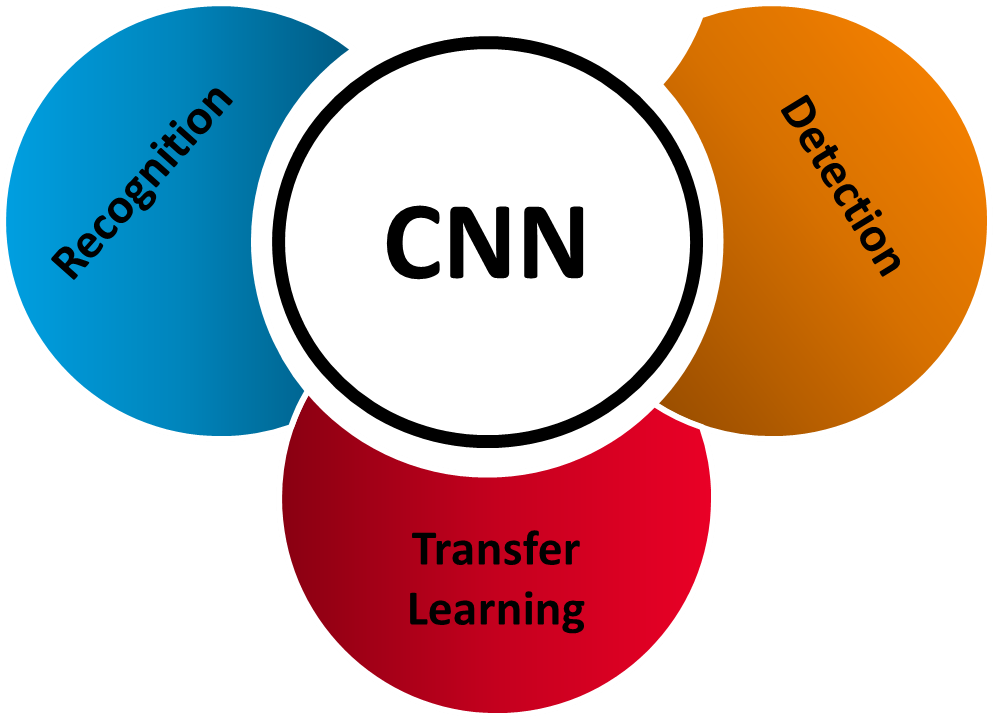
\includegraphics[width=8cm]{pics/mind_map}
	\caption{Mind map penelitian terdahulu terkait CNN}
	\label{fig:mind_map}
\end{figure}\\
Dalam penelitian terdahulu, yang dilakukan Yizhang, Bailing dan frans (Yizhang Xia, Bailing Zhang \& Frans Coenen, 2015), menjelaskan bahwa CNN dapat dilakukan proses secara multi-task learning. Kasus penelitian yang diambil adalah deteksi wajah dengan teknik oklusi objek-objek yang ada pada wajah, kemudian dilakukan proses learning terhadap tiap objek sehingga terjadi multi-task learning. Perbedaan yang dilakukan penelitian ini adalah banyak penelitian sebelumnya yang menggunakan pendekatan lokalisasi, segmentasi, ekstraksi fitur dan pengenalan objek. \\
Penelitian lainnya yang dilakukan Earnest Paul dan Krishna (Earnest Paul Ijjina \& C Krishna Mohan, 2015) meneliti penegalan human action menggunakan MOCAP (Motion Capture) dengan Fuzzy Convolution Neural Network. Informasi MOCAP digunakan untuk menghitung variasi pergerakan yang terpisah dan kemudian digabungkan selama proses eksekusi. Fungsi keanggotaan fuzzy digunakan untuk melakukan ekstraksi fitur dengan menggabungkan pose yang berasosiasi dengan aksi yang dilakukan manusia.\\
Penelitian lainnya yang dilakukan Lin, Hsu dan Chen (Hsien-I Lin, Ming-Hsiang Hsu \& Wei-Kai Chen, 2015) untuk melakukan deteksi terhadap gesture pergarakan dari tangan. Untuk meningkatkan performa, penelitian ini melakukan pemodelan dari kulit dan kalibrasi terhadap posisi dan orientasi dari objek. Untuk menghilangkan noise pada gambar, ditambah pendekatan Gaussian Mixture model (GMM) untuk melakukan training dalam menghadapi permasalahan noise yang diakibatkan cahaya yang berpengaruh terhadap warna kulit. Kalibrasi terhadap posisi dan orientasi objek digunakan untuk proses translasi dan rotasi objek sehingga menjadi pose yang netral. Hasil dari kalibrasi akan digunakan untuk CNN dan menghasilkan akurasi 95.96\% untuk pengenalan 7 variasi gesture dari tangan.\\
Penelitian terkait CNN adalah mengenai transfer learning dengan CNN yang dilakukan oleh Yejun Tang, Liangrui Peng, Qian Xu, Yanwei Wang \& Akio Furuhata. Transfer learning pada CNN digunakan untuk menyelesaikan kasus OCR untuk pengenalan huruf cina. Model transfer learning yang diuji terbagi menjadi 2 arsitektur CNN yaitu T \& L dengan prosedur:
\begin{enumerate}
	\item CNN L dilakukan training untuk melakukan ekstraksi fitur dan batasan klasifikasi.
	\item Bobot hasil pembelajaran CNN L disalurkan kepada CNN T untuk diinisialisasi.
	\item Layer Fully-Connected dari CNN T dikembangkan dengan beberapa sampel pada domain target untuk menyeimbangkan domain awal dan target, dimana layer konvolusi dan subsampling tetap sama seperti sebelumnya dari CNN L.
\end{enumerate}
Hasil dari penelitian transfer learning memberikan akurasi hingga  88.56\%  dengan variasi font Kai Ti (kt) and Song Ti (st).\\
Penelitian-penelitian terdahulu yang telah dijelaskan di atas dapat dituliskan dalam sebuah matriks literatur yang dapat dilihat pada tabel 2.1 sebagai berikut.
\begin{table}
	\centering
	\caption{Matriks literatur penelitian terdahulu yang berhubungan dengan penelitian Convolution Neural Network}
	\label{tab:tab1}
	\begin{tabular}{ |m{2cm}|m{7cm}|m{1cm}|m{1cm}| } 
		\hline
		Judul & \multicolumn{3}{|m{13cm}|}{Face Occlusion Detection Based on Multi-task Convolution Neural Network} \\
		\hline
		Pengarang & \multicolumn{3}{|m{13cm}|}{Yizhang Xia, Bailing Zhang, Frans Coenen} \\ 
		\hline
		Tahun & \multicolumn{3}{|m{13cm}|}{2015} \\ 
		\hline
		Metode & \multicolumn{3}{|m{13cm}|}{Pre training, Fine tuning \& Multi task predicting}\\
		\hline
		Kontribusi  & \multicolumn{3}{|m{13cm}|}{ConvNets model \& A large face occlusion database}\\ 
		\hline
		Pekerjaan Mendatang  & \multicolumn{3}{|m{13cm}|}{Peningkatan model menggunakan weakly-supervised learning, yang lebih realistis dalam dunia nyata} \\		
		\hline\hline
		
		Judul & \multicolumn{3}{|m{13cm}|}{Human Action Recognition based on Motion Capture Information using Fuzzy Convolution Neural Networks} \\
		\hline
		Pengarang & \multicolumn{3}{|m{13cm}|}{Earnest Paul Ijjina, C Krishna Mohan} \\ 
		\hline
		Tahun & \multicolumn{3}{|m{13cm}|}{2015} \\ 
		\hline
		Metode & \multicolumn{3}{|m{13cm}|}{Motion capture (MOCAP) information using a Fuzzy convolutional neural network}\\
		\hline
		Kontribusi  & \multicolumn{3}{|m{13cm}|}{High classification accuracy can be achieved by extracting features using fuzzy membership functions and MOCAP information of only three human joints}\\ 
		\hline
		Pekerjaan Mendatang  & \multicolumn{3}{|m{13cm}|}{Extensive experimentation on other MOCAP datasets \& Datasets with predicted human joint information like JHMDB, to identify the set of features suitable for action recognition across multiple datasets} \\ 
		\hline\hline
		
		Judul & \multicolumn{3}{|m{13cm}|}{Human Hand Gesture Recognition Using a Convolution Neural Network} \\
		\hline
		Pengarang & \multicolumn{3}{|m{13cm}|}{Hsien-I Lin, Ming-Hsiang Hsu, and Wei-Kai Chen} \\ 
		\hline
		Tahun & \multicolumn{3}{|m{13cm}|}{2014} \\ 
		\hline
		Metode & \multicolumn{3}{|m{13cm}|}{Convolution neural network (CNN) method to recognize hand gestures of human task activities from a camera image, Gaussian Mixture model (GMM) to train the skin model which is used to robustly filter out non-skin colors of an image and the calibration of hand position and orientation aims at translating and rotating the hand image to a neutral pose
			}\\
		\hline
		Kontribusi  & \multicolumn{3}{|m{13cm}|}{}\\ 
		\hline
		Pekerjaan Mendatang  & \multicolumn{3}{|m{13cm}|}{A high-level semantic analysis will be applied to the current system to enhance the recognition capability for complex human tasks} \\ 
		\hline\hline
		
		Judul & \multicolumn{3}{|m{13cm}|}{A Convolution Neural Network Based Variational Restoration Model} \\
		\hline
		Pengarang & \multicolumn{3}{|m{13cm}|}{Xinyan Yu, Guohao Lyu, Siwei Luo, Junbo Liu} \\ 
		\hline
		Tahun & \multicolumn{3}{|m{13cm}|}{2015} \\ 
		\hline
		Metode & \multicolumn{3}{|m{13cm}|}{Convolution neural network for Extracting and expressing the features \& Convolution neural network to get classification of features
		}\\
		\hline
		Kontribusi  & \multicolumn{3}{|m{13cm}|}{Improving Convolution Neural Network with regularization restoration}\\ 
		\hline
		Pekerjaan Mendatang  & \multicolumn{3}{|m{13cm}|}{Finding effective features and the segmentation of image patch for better restoring image} \\
	\end{tabular}
\end{table}

%-----------------------------------------------------------------------------%
\section{\f{Feedforward Neural Network}} \label{fnn}
%-----------------------------------------------------------------------------%
Di dalam \f{machine learning}, \f{artificial neural network} (ANN) adalah model yang terinspirasi oleh \f{neural network} biologis. \f{Aritificial neural network} dapat melakukan estimasi atau aproksimasi fungsi non-linear dengan nilai \f{output} yang dapat berupa nilai \f{real}, diskret, atau vektor. Pada alamnya, neuron menerima sinyal melalui sinaps yang terletak pada dendrit. Neuron akan teraktivasi dan dapat meneruskan sinyal apabila sinyal yang diterima memenuhi batas tertentu. Sinyal tersebut dapat diterima sinaps lain dan dapat mengaktivasi neuron lainnya. Beberapa permasalahan yang dapat diselesaikan dengan ANN diantaranya adalah klasifikasi, kategorisasi, aproksimasi fungsi, dan prediksi .

\f{Feedforward neural network} adalah salah satu jenis ANN. \f{Feedforward neural network} terdiri dari beberapa unit yang dikelompokkan dalam \f{layer} di mana setiap \f{layer} yang bersebelahan saling terhubung melalui suatu unit. Pada \f{feedforward neural network}, koneksi antar \f{unit} tidak membentuk \f{cycle} seperti yang ada pada \f{recurrent neural network}. Kalkulasi \f{feedforward neural network} dari \f{input} ke \f{output} berjalan ke satu arah sesuai dengan strukturnya yang tampak seperti graf berarah. Contoh \f{feedforward neural network} dengan satu \f{hidden layer} dapat dilihat pada Gambar \ref{fig:fnn} berikut.

\begin{figure}
	\centering
	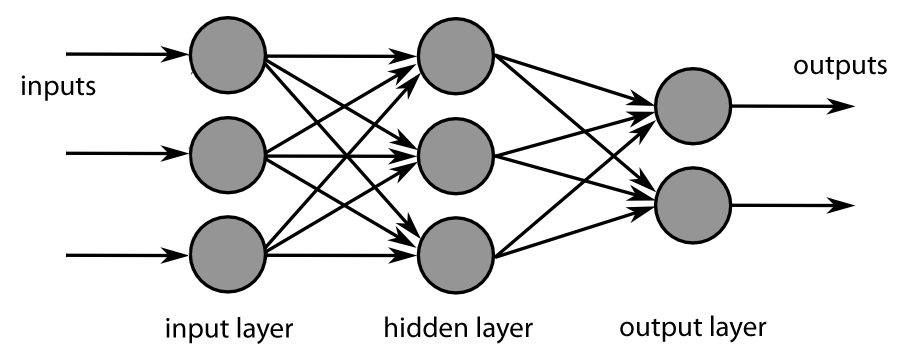
\includegraphics[width=0.8\textwidth,height=0.3\textwidth]
	{pics/fnn.png}
	\caption{Contoh \f{feedforward neural network}}
	\label{fig:fnn}
\end{figure}
\vspace{-1.2cm}
\begin{center}
	{\small Sumber gambar: http://technobium.com/stock-market-prediction-using-neuroph-neural-networks/}
\end{center}

\f{Feedforward neural network} terdiri dari \f{input layer}, \f{output layer}, dan beberapa \f{hidden layer} apabila dibutuhkan. Jumlah \f{hidden layer} berperan pada seberapa kompleks batas keputusan yang dapat dibentuk oleh \f{network} seperti pada Gambar \ref{fig:hl}.

\begin{figure}
	\centering
	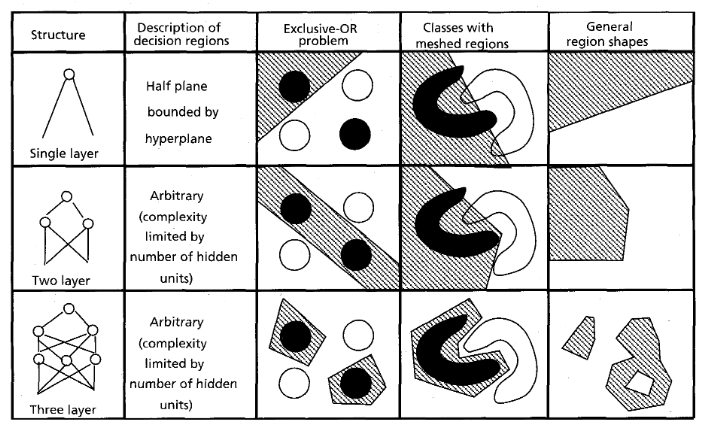
\includegraphics[width=1\textwidth,height=0.6\textwidth]
	{pics/hl.png}
	\caption{Interpretasi geometris pada peran \f{hidden layer}}
	\label{fig:hl}
\end{figure}
\vspace{-1.2cm}
\begin{center}
	{\small Sumber gambar: \cite{paper.jain}}
\end{center}

Pada \f{input layer}, jumlah unit atau neuron yang ada sesuai dengan jumlah elemen yang ada pada vektor \f{input}. Begitu juga dengan \f{output layer}, jumlah unit yang ada sesuai dengan banyaknya elemen yang diinginkan pada vektor \f{output}. Berbeda dengan \f{input layer} dan \f{output layer}, jumlah unit dalam \f{hidden layer} sifatnya bebas. Setiap unit menghasilkan suatu \f{output} dari kombinasi linear beberapa nilai \f{input} dengan bobotnya masing-masing. Hasil dari kombinasi linear tersebut kemudian diaktivasi dengan fungsi aktivasi. Proses ini dapat dilihat pada Rumus \ref{equ:perceptron}.

\begin{equation}
\label{equ:perceptron}
y(x) = g\left(\sum\limits_{i=1}^{n} w_{ij}x_{i} + w_{0j}\right)
\end{equation}

\begin{itemize}
	\item $x$ merupakan vektor \f{input}
	\item $w$ merupakan vektor bobot
	\item $w_{ij}$ merupakan bobot yang menghubungkan unit ke-\f{i} pada \f{layer} sebelumnya dan unit ke-\f{j} pada \f{layer} saat itu
	\item $w_{0j}$ merupakan bobot untuk bias
	\item $g$ merupakan fungsi aktivasi
\end{itemize}

Pada Rumus \ref{equ:perceptron} vektor \f{input} pada suatu \f{layer} bergantung pada \f{output} di \f{layer} sebelumnya, kecuali untuk \f{layer} pertama yaitu \f{input layer}. Fungsi aktivasi $g$ dapat berbeda untuk setiap \f{layer}, tapi pada umumnya sama untuk setiap unit pada \f{layer} yang sama. Pada penelitian ini fungsi aktivasi yang digunakan adalah \f{rectified linear unit} (ReLU) yang dapat dilihat pada Rumus \ref{equ:relu}, dan \f{sigmoid} pada Rumus \ref{equ:sigmoid}.

\begin{equation}
\label{equ:relu}
g(x) = max(0, x)
\end{equation}

\begin{equation}
\label{equ:sigmoid}
g(x) = \frac{1}{1 + e^{-x}}
\end{equation}

Pada Rumus \ref{equ:perceptron} terdapat $w_{0j}$ yang merupakan bobot untuk bias. Bias bersifat seperti konstanta yang selalu bernilai +1, sehingga pengaruh bias tergantung pada bobotnya.

%-----------------------------------------------------------------------------%
\section{Convolution Neural Network (CNN)}
%-----------------------------------------------------------------------------%
CNN merupakan salah satu variasi dari multilayer perceptron (MLP). Keuntungan dari metode CNN, khsusnya untuk kasus pengenalan pola dibandingkan pendekatan konvensional adalah kemampuan untuk mengurangi dimensi data, ekstraksi fitur secara sekuensial, dan mengklasifikasi salah satu struktur jaringan. Arsitektur dasar dari model CNN terinspirasi dari visual cortex yang dikenalkan oleh hubel dan wiesel pada tahun 1962.\\
Pada tahun 1980, neocognitron fukushima membuat pertama kali komputasi menggunakan model CNN, dan kemudian pada tahun 1989, dengan menggunakan model yang ditemukan fukushima, LeCun menemukan performa dari beberapa proses untuk pengenalan pola menggunakan metode error gradient.\\
Model CNN yang digunakan oleh LeCun merupakan pengembangan dari MLP tradisional yang didasari 3 ide, local receptive field, weight sharing dan spatial subsampling. Ide dasar ini diorganisir kedalam 2 tipe layer, yaitu convolution dan subsampling layer. Seperti yang ditunjukan gambar 1, digunakan 3 convolution layer dengan kombinasi layer subsampling dan 1 output layer. Layer convolution dan subsampling tersusun kedalam plane atau disebut feature maps.\\
\f{Convolutional neural network} (CNN) adalah salah satu tipe \f{feedforward neural network} yang terinspirasi dari cara kerja visual korteks. Berdasarkan penelitian , korteks visual terdiri dari banyak sel kompleks. Sel-sel ini disebut \f{receptive field} dan sensitif terhadap bagian kecil bidang visual. Salah satu sifat yang dimiliki CNN adalah \f{sparse connectivity}. \f{Sparse connectivity} memungkinkan suatu \f{layer} saling terhubung hanya dengan unit-unit terdekat. Dengan kata lain, \f{input} dari suatu unit merupakan \f{subset} dari unit pada \f{layer} sebelumnya. Ilustrasi \f{sparse connectivity} dapat dilihat pada Gambar.

\begin{figure}
	\centering
	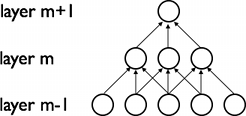
\includegraphics[width=0.45\textwidth,height=0.2\textwidth]
	{pics/sparse.png}
	\caption{\f{Sparse Connectivity}}
	\label{fig:sparse}
\end{figure}
\vspace{-1.2cm}
\begin{center}
	{\small Sumber gambar: http://deeplearning.net/tutorial/lenet.html}
\end{center}

Tumpukan \f{layer} pada Gambar \ref{fig:sparse} hanya memiliki satu unit pada \f{layer} $m + 1$. Hal ini merepresentasikan unit atau bagian-bagian kecil yang ada pada \f{layer} $m - 1$ bagaikan disaring atau di-\f{filter} hingga \f{layer} $m + 1$ memahami bidang visual secara utuh. 

Selain \f{sparse connectivity}, CNN juga memiliki sifat \f{shared weights}. Setiap \f{layer} kecuali \f{output layer} memiliki \f{filter} yang fungsinya untuk menyaring bagian kecil dari bidang visual. \f{Filter} tersebut direplikasi dengan bobot yang sama ke seluruh bidang visual dengan untuk menyaring unit atau bagian-bagian kecil sehingga membentuk \f{feature map}. Pada Gambar \ref{fig:shared} berikut, lima unit pada \f{layer} $m - 1$ disaring dengan \f{filter} berukuran tiga, sehingga membentuk tiga unit \f{feature map}. Garis yang berwarna sama menandakan bobot yang sama.

\begin{figure}
	\centering
	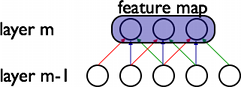
\includegraphics[width=0.45\textwidth,height=0.15\textwidth]
	{pics/shared.png}
	\caption{\f{Shared weights} untuk \f{filter} yang sama}
	\label{fig:shared}
\end{figure}
\vspace{-1.2cm}
\begin{center}
	{\small Sumber gambar: http://deeplearning.net/tutorial/lenet.html}
\end{center}

Untuk merepresentasikan data atau bidang visual yang kompleks, setiap \f{layer} pada CNN dapat mempunyai beberapa \f{feature map} atau \f{channel}. Rumus untuk menghitung \f{feature map} ke-$k$ pada \f{pixel} koordinat $(i,j)$ yang ditentukan oleh bobot $W^{k}$ dan bias $b_{k}$ adalah sebagai berikut.

\begin{equation}
\label{equ:featuremap}
y^{k}_{ij} = g\left((W^{k} * x)_{ij} + b_{k}\right)
\end{equation}

Setiap \f{feature map} pada layer $m - 1$ berkontribusi dalam menentukan nilai \f{feature map} $k$ pada layer $m$. Dengan kata lain, setiap \f{pixel} yang berada dalam \f{feautre map} $k$ nilainya akan ditentukan oleh seluruh \f{pixel} yang terhubung, pada \f{feature map} di \f{layer} $m - 1$. Pada ilsutrasi Gambar \ref{fig:featuremap}, \f{layer} $m$ memiliki dua \f{feature map} $y^0$ dan $y^1$. \f{Pixel} (kotak berwarna biru) pada $y^0$ ditentukan dari 2x2 \f{pixel} yang terhubung dengan bobot $W^{kl}_{ij}$. $W^{kl}_{ij}$ menyatakan bobot yang menghubungkan \f{pixel} koordinat $(i,j)$ pada \f{feature map} ke-$l$ di \f{layer} $m - 1$ ke \f{pixel} yang terhubung pada \f{feature map} ke-$k$ di \f{layer} $m$.

\begin{figure}
	\centering
	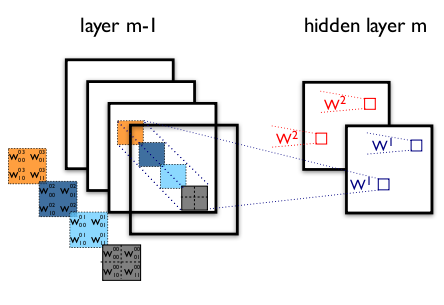
\includegraphics[width=0.9\textwidth,height=0.55\textwidth]
	{pics/featuremap.png}
	\caption{Ilustrasi \f{layer} pada \f{convolutional neural network}}
	\label{fig:featuremap}
\end{figure}
\vspace{-1.2cm}
\begin{center}
	{\small Sumber gambar: http://deeplearning.net/tutorial/lenet.html}
\end{center}

\f{Convolutional Neural Network} biasanya terdiri dari beberapa \f{filter} atau disebut juga dengan \f{convolutional layer}, sering kali diikuti denga \f{subsampling layer} dan diakhiri dengan \f{fully connected layers}. Terdapat juga jenis CNN yang tidak diakhiri dengan \f{fully connected layers} melainkan \f{convolutional layer} lainnya yang mempertahankan dimensi data dalam bentuk citra 2D. CNN jenis ini disebut dengan \f{Fully Convolutional Neural Network}.

\subsection{Convolutional Layer}
Pada layer convolution, tiap neuron terhubung secara local kepada area yang lebih kecil (local receptive field) pada layer sebelumnya. Semua neuron yang memiliki feature maps yang sama memperoleh data dari input area yang berbeda hingga semua input plan tersaring tetapi saling berbagi bobot (weight sharing).\\
\f{Convolutional layer} memiliki tiga \f{hyperparameter} yang mengatur transformasi \f{feature map} yang dihasilkan: \f{depth} $D$, \f{stride} $S$, dan \f{zero-padding} $P$. Dalam tahap \f{feedforward}, \f{convolutional layer} berukuran $F$ akan bergeser pada gambar berukuran $W$, dan menghasilkan \f{feature map} sebanyak $D$ dengan ukuran $W'$ yang dapat dihitung menggunakan Rumus \ref{equ:convlayer} berikut.

\begin{equation}
\label{equ:convlayer}
W' = (W - F + 2P) / S + 1
\end{equation}

Dalam praktiknya, \f{zero-padding} sering kali digunakan untuk menyesuaikan ukuran hasil \f{feature map}. \f{Zero padding} dengan ukuran $P = (F - 1)/2$ dipastikan menghasilkan \f{feature map} dengan ukuran yang sama dengan \f{feature map} sebelumnya apabila \f{stride} $S = 1$. \f{Deep learning framework} seperti \f{theano} menyebut \f{padding} dengan sifat tersebut sebagai \f{same padding} . Terdapat juga \f{full padding} yang menghasilkan \f{feature map} dengan ukuran $W' = W + F - 1$.

\subsection{Subsampling Layer}
Pada layer subsampling, feature maps didownsampling secara spasial, dimana ukuran map dikurangi berdasarkan 2 faktor. Contohnya, feature map pada layer C3 dengan ukuran 10x10 dilakukan subsampling untuk menyesuaikan feature map dengan ukuran 5x5 pada layer selanjutnya. Layer terakhir adalah F6 yang merupakan proses klasifikasi.
Dalam arsitektur \f{convolutional neural network}, \f{pooling layer} berfungsi untuk mereduksi ukuran spasial gambar secara bertahap sehingga mengurangi parameter dan komputasi pada \f{network}. \f{Pooling layer} menerima \f{input} \f{feature map} berukuran $W_{1}$ sebanyak $D_{1}$ dan parameter ukuran \f{pooling} $F$ dan \f{stride} $S$. Sama halnya dengan \f{convolutional layer}, \f{pooling layer} juga bergeser terhadap input dan menghasilkan \f{feature map} berjumlah $D_{2} = D_{1}$ dengan ukuran $W_{2} = (W_{1} - F)/S + 1$. Terdapat beberapa jenis \f{pooling layer}, dan yang paling sering digunakan adalah:

\begin{enumerate}
	\item \f{Max Pooling} \\
	Dalam \f{pooling} berukuran $F$, \f{Max pooling} akan mengambil hasil aktivasi yang terbesar dalam daerah yang termasuk pada pergeseran saat itu. Ilustrasi ini dapat dilihat pada Gambar \ref{fig:maxpool} berikut dengan $F = 2$ dan $S = 2$.
	
	\begin{figure}
		\centering
		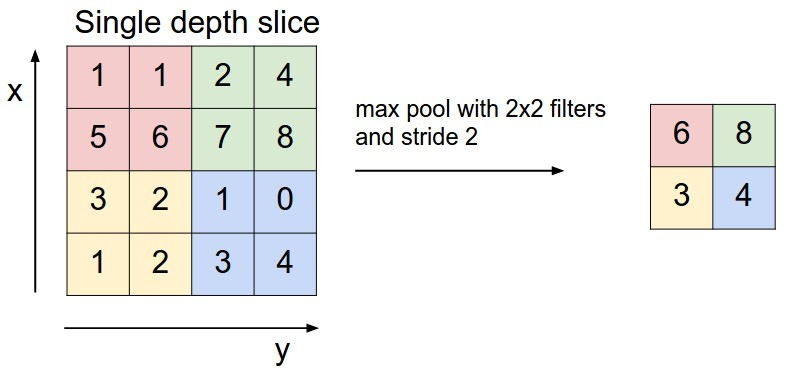
\includegraphics[width=0.8\textwidth,height=0.35\textwidth]
		{pics/maxpool.jpeg}
		\caption{Ilustrasi \f{max pooling}}
		\label{fig:maxpool}
	\end{figure}
	\vspace{-1.2cm}
	\begin{center}
		{\small Sumber gambar: http://cs231n.github.io/convolutional-networks}
	\end{center}
	
	\item \f{Average Pooling} \\
	Berbeda dengan \f{max pooling}, \f{average pooling} mengambil hasil aktivasi pada daerah \f{filter} dan menghitung rata-rata dari seluruh hasil aktivasi dalam daerah tersebut.
\end{enumerate}
%-----------------------------------------------------------------------------%
\subsection{\f{Fully Connected Layer}}
%-----------------------------------------------------------------------------%
\f{Fully connected layer} adalah \f{feed forward neural network} yang dijelaskan pada subbab \ref{fnn}. Biasanya, \f{fully connected layer} berada pada \f{layer} akhir pada arsitektur \f{convolutional neural network} dan bertujuan untuk memproses hasil \f{feature extraction} yang dilakukan pada \f{layer} sebelumnya menjadi suatu \f{output} tertentu. Gambar \ref{fig:cnnlayers} berikut merupakan contoh arsitektur dengan susunan \f{convolutional layer}, \f{pooling layer}, dan \f{fully connected layer}.

\begin{figure}
	\centering
	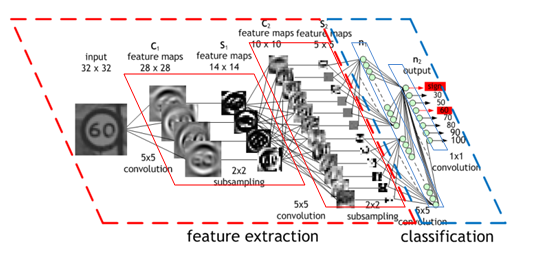
\includegraphics[width=1\textwidth,height=0.45\textwidth]
	{pics/cnnlayers.png}
	\caption{Contoh arsitektur \f{convolutional neural network}}
	\label{fig:cnnlayers}
\end{figure}
\vspace{-1.2cm}
\begin{center}
	{\small Sumber gambar: https://devblogs.nvidia.com}
\end{center}
%-----------------------------------------------------------------------------%
\section{\f{Backpropagation}}
%-----------------------------------------------------------------------------%
Tujuan dari melatih model \f{feedforward neural network} adalah membuat model tersebut dapat memprediksi nilai dengan galat seminimal mungkin. \f{Feedforward neural network} menggunakan metode \f{backpropagation} untuk melatih nilai bobot-bobot pada \f{network} tersebut. Untuk melatih suatu bobot, metode ini melakukan \f{propagation} dari galat pada \f{output layer} sehingga informasi ini tersebar ke \f{layer} sebelumnya untuk digunakan dalam mengubah bobot.

Untuk $\delta^{(l+1)}$ sebagai galat pada \f{layer} $l+1$ dengan fungsi galat $J(W,b;x,y)$ di mana $W,b$ adalah parameter, dan $x,y$ adalah pasangan \f{input} dan label, apabila \f{layer} $l$ dan \f{layer} $l+1$ saling terhubung maka galat pada \f{layer} $l$ adalah sebagai berikut.


\begin{equation}
\begin{aligned}
\delta^{(l)} &= ((W^{(l)})^{T}\delta^{(l+1)}) \cdot f'(z^{(l)}) \\
f'(z^{(l)}) &= a^{(l)} \cdot (1-a^{(l)})
\end{aligned}
\end{equation}

\begin{equation}
\label{equ:erder}
\begin{aligned}
\Delta_{w^{(l)}}J(W,b;x,y)&=\delta^{(l+1)}(a^{(l)})^{T} \\
\Delta_{b^{(l)}}J(W,b;x,y)&=\delta^{(l+1)}
\end{aligned}
\end{equation}

Pada \f{convolutional layer} dan \f{pooling layer}, galat pada \f{layer} $l$ dihitung dengan fungsi \f{upsample} $g(x)$ tergantung pada \f{layer} yang digunakan.

\begin{equation}
\label{equ:errorc}
\delta^{(l)}_{k} = upsample((W^{(l)}_{k})^{T}\delta^{(l+1)}_{k}) \cdot f'(z^{(l)}_{k}) 
\end{equation}

\[
g(x)
\begin{cases}
\frac{\sum_{k=1}^{m} x_{k}}{m}, \frac{\delta g}{\delta x} = \frac{1}{m}, & \text{average pooling} \\
max(x), \frac{\delta g}{\delta x} =
\begin{cases}
1, & \text{if } x_{i} = max(x) \\
0, & otherwise
\end{cases}
, & \text{max pooling}
\end{cases}
\]

\begin{center}
	{\small Sumber rumus: http://www.slideshare.net/kuwajima/cnnbp}
\end{center}

Rumus \ref{equ:erder} digunakan untuk mengubah bobot pada suatu \f{layer}. Salah satu cara untuk mengubah bobotnya adalah dengan \f{stochastic gradient descent} yang menggunakan Rumus \ref{equ:sgd} berikut.

\begin{equation}
\label{equ:sgd}
\theta = \theta-\alpha\Delta_{\theta}J(\theta;x^{(i)},y^{(i)})
\end{equation}

\begin{center}
	{\small Sumber rumus: http://ufldl.stanford.edu/tutorial/supervised/ConvolutionalNeuralNetwork}
\end{center}


%-----------------------------------------------------------------------------%
\section{Algoritma Optimasi}
%-----------------------------------------------------------------------------%
Algoritma optimasi digunakan untuk permasalahan meminimalisasi \f{loss}. Untuk \f{dataset} $D$, objektif dari optimasi adalah rata-rata $loss$ $|D|$ dari seluruh anggota \f{dataset} $D$. Dengan $fw(X^{(i)})$ adalah galat pada data ke $X^{(i)}$, dan $r(W)$ adalah regularisasi dengan bobot $\lambda$, maka galat rata-rata dapat dihitung menggunakan Rumus \ref{equ:avgloss} berikut .

\begin{equation}
\label{equ:avgloss}
L(W)=\frac{1}{|D|}\sum\limits_{i}^{|D|}fw(X^{(i)})+\lambda r(W)
\end{equation}

Karena $|D|$ pada kenyataannya dapat bernilai sangat besar, dalam praktiknya setiap iterasi menggunakan aproksimasi secara stokastik dengan memilih $N << |D|$ sehingga galat rata-rata dihitung dengan Rumus \ref{equ:avgloss2} berikut .

\begin{equation}
\label{equ:avgloss2}
L(W)\approx\frac{1}{N}\sum\limits_{i}^{N}fw(X^{(i)})+\lambda r(W)
\end{equation}
%-----------------------------------------------------------------------------%
\subsection{\f{Stochastic Gradient Descent} (SGD)}
%-----------------------------------------------------------------------------%
\f{Stochastic gradient descent} mengubah bobot $W$ dengan kombinasi linear dari \f{gradient} negatif $\Delta L(W)$ dan perbaharuan bobot $V_{t}$ pada iterasi sebelumnya. Untuk menghitung nilai perbaharuan $V_{t+1}$ dan bobot $W_{t+1}$ pada iterasi $t+1$ digunakan Rumus \ref{equ:sgd2} dan \ref{equ:sgd2-3} berikut .

\begin{equation}
\label{equ:sgd2}
V_{t+1} = \mu V_{t} - \alpha \Delta L(W_{t})
\end{equation}

\begin{equation}
\label{equ:sgd2-3}
W_{t+1} = W_{t} + V_{t+1}
\end{equation}
%-----------------------------------------------------------------------------%
\subsection{\f{Nesterov's Accelerated Gradient} (Nesterov)}
%-----------------------------------------------------------------------------%
\f{Nesterov's accelerated gradient} (Nesterov) diusulkan oleh Nesterov sebagai metode optimal untuk optimasi, dengan laju konvergensi mencapai $O(1/t^{2})$. Dalam praktiknya, Nesterov dapat menjadi metode yang cukup efektif untuk mengoptimasi arsitektur \f{deep learning} tertentu, seperti yang didemonstrasikan oleh  dalam membuat \f{autoencoders}. Perubahan bobot dalam algoritma Nesterov menggunakan Rumus berikut .

\begin{equation}
\label{equ:nesterov}
V_{t+1}=\mu V_{t} - \alpha\Delta L(W_{t} + \mu V_{t})
\end{equation}

\begin{equation}
W_{t+1} = W_{t} + V_{t+1}
\end{equation}

Perbedaan Nesterov dengan SGD terdapat pada penambahan momentum dalam menghitung \f{gradient} $\Delta L(W_{t} + \mu V_{t})$. Dalam SGD, perhitungan \f{gradient} $\Delta L(W_{t})$ hanya mengambil bobotnya saja.

%-----------------------------------------------------------------------------%
\section{Fungsi Galat}
%-----------------------------------------------------------------------------%
Fungsi galat adalah fungsi yang menghitung galat dari hasil prediksi $\hat{y}$ dengan nilai $y$ yang sebenarnya. Pada penelitian ini, penulis menggunakan dua jenis fungsi galat, yakni \f{cross-entropy loss} (Rumus \ref{equ:cl}) dan \f{euclidean loss} (L2) (Rumus \ref{equ:el}). Dilihat dari fungsinya, \f{cross entropy} bekerja lebih agresif dalam memperbaiki dibandingkan dengan \f{euclidean error}.

\begin{equation}
\label{equ:cl}
crossentropy(y, \hat{y}) = -(y * log(\hat{y}) + (1 - y) * log(1 - \hat{y}))
\end{equation}

\begin{equation}
\label{equ:el}
euclideanloss(y, \hat{y}) = \frac{1}{2} \|y - \hat{y}\|^{2}_{2}
\end{equation}
\begin{center}
	{\small Sumber rumus: http://caffe.berkeleyvision.org}
\end{center}
%-----------------------------------------------------------------------------%
\section{Deeplearning4j}
%-----------------------------------------------------------------------------%
Deeplearning4j adalah library yang berbasis teknologi JAVA yang mampu terintegrasi dengan Hadoop, Spark, DL4J diciptakan untuk digunakan dalam lingkungan bisnis daripada untuk riset.\\
Deeplearning4j bertujuan memiliki fungsi pembelajaran mesin untuk penggunaan yang siap pakai, sehingga membantu pembuatan prototipe aplikasi yang lebih cepat untuk pengguna selain akademisi atau pelaku riset. Deeplearning4j memiliki lisensi Apache 2 yang dimiliki oleh pembuatnya.\\
Deeplearning4j merupakan framework yang mampu melakukan proses secara pada lingkungan sistem yang terdistribusi, kemampuan multi-thread maupun single-thread. Ketika melakukan proses training pada lingkungan cluster, dimana proses komputasi dilakukan untuk data besar mampu dilakukan secara lebih cepat. Proses training dilakukan secara paralel dengan mengurangi iterasi dan memiliki kompatibilitas dengan JAVA, SCALA dan CLOJURE. Deeplearning4j berperan sebagai komponen modular dalam komponen yang terbuka sehingga menjadi framework pertama yang mengadaptasi arsitektur micro-service.
\begin{figure}[htp]
	\centering
	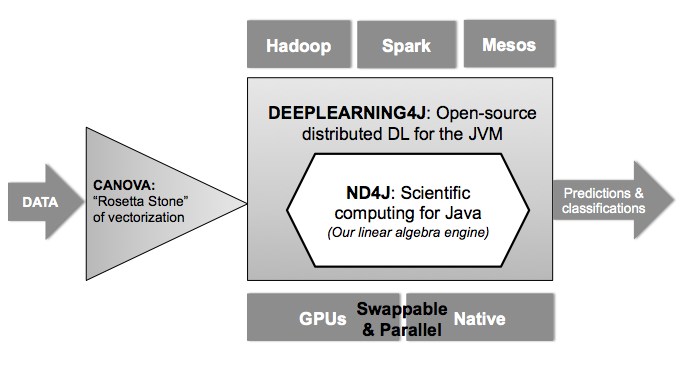
\includegraphics[width=8cm]{pics/dl4j}
	\caption{Mind map penelitian terdahulu terkait CNN}
	\label{fig:dl4j}
\end{figure}\\

%-----------------------------------------------------------------------------%
\section{Web Service}
%-----------------------------------------------------------------------------%
Teknologi Web Service adalah teknologi yang mengadopsi SOA (Software Oriented Architecture). Pada web service, user mengirimkan request kepada web service dan web service akan memberikan respon terkait request user tersebut. Agar user bisa berkomunikasi dengan web service, digunakan standard komunikasi yang biasa disebut WSDL (Web Service Description Language). WSDL membentuk spesifikasi dasar komunikasi dari suatu web service dengan:
\begin{enumerate}
	\item Penyedia service mendeskripsikan fungsi menggunakan WSDL. Definisi tersebut dipublikasi pada repositori layanan. Repositori bisa menggunakan UDDI. Bentuk lain dari direktori juga bisa digunakan.
	\item User dari layanan melakukan request kepada repositori untuk menemukan service dan memberikan aturan bagaimana berkomunikasi dengan service tersebut. Bagian dari WSDL yang disediakan oleh penyedia diberikan kepada user. Hal ini akan memberikan informasi kepada user bagaimana bentuk request dan hasil respon yang akan diberikan oleh service.
	\item User menggunakan WSDL untuk mengirimkan request kepada penyedia service
	\item Penyedia service menyediakan respon kepada user
\end{enumerate}

Android merupakan sistem operasi untuk teknologi mobile yang sudah digunakan secara umum. Penggunaaan smartphone berbasis android sudah bukan lagi menjadi barang baru karena kemajuan teknologi sehingga menjadikan harga smartphone menjadi terjangkau dan dapat mengjangkau semua elemen masyarakat.

%-----------------------------------------------------------------------------%
\section{Batik}
%-----------------------------------------------------------------------------%
Indonesia merupakan negara kepulauan yang memiliki banyak suku dan ras dan sehingga memiliki keanekaram bahasa, budaya dan kebiasaan. Salah satu keunikan yang dimiliki Indonesia adalah memiliki keanekaragaman jenis kain yang berasal dari tiap daerah, diantaranya batik, tok wie, kain dodot, kain panjang dll.\\
\begin{figure}[htp]
	\centering
	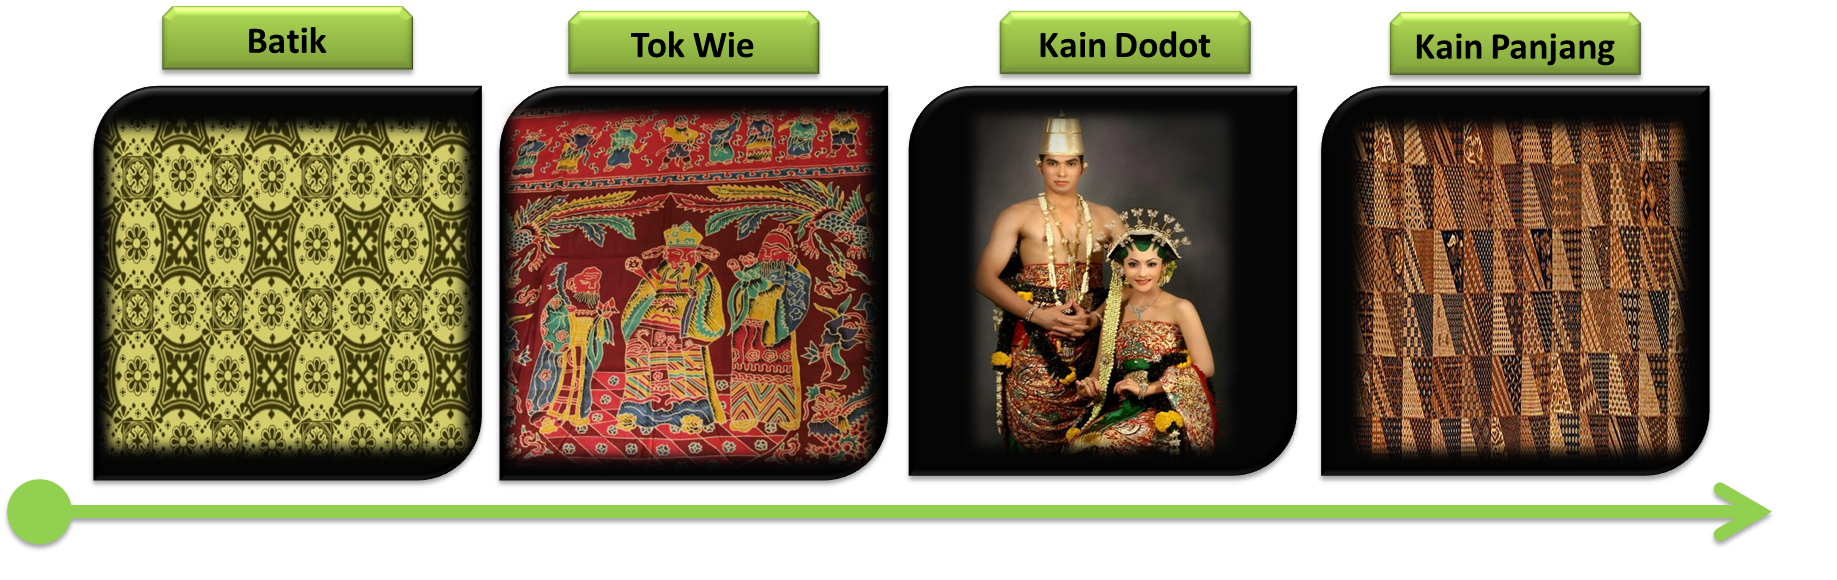
\includegraphics[width=10cm]{pics/kain_indonesia}
	\caption{Contoh kain dari berbagai daerah di indonesia}
	\label{fig:kain_indonesia}
\end{figure}\\
Salah satu kain tradisional Indonesia adalah batik. Batik merupakan kain bergambar yang memiliki gaya, warna dan tekstur dimana proses pembuatannya dilakukan secara manual maupun menggunakan mesin. Batik memiliki beberapa motif seperti motif kawung, motif parangkusumo, motif truntum, motif tambal, motif pamiluto, motif parang, motif liris maupun motif udan nitik.
